%Stil på uppsats
\documentclass[11pt]{article}
\usepackage[utf8]{inputenc}
\usepackage[swedish]{babel}
\usepackage{verbatim}
\renewcommand{\baselinestretch}{1.3}
\renewcommand{\arraystretch}{1}

%Skippa indrag av brödtext
\usepackage{parskip}

%Bilder sida vid sida
\usepackage{subfig}

% Formattera text
\usepackage[text={13cm,22cm}]{geometry}

\usepackage{booktabs}
\usepackage{floatrow}
\floatsetup[table]{capposition=top}
\usepackage{amsmath}
\usepackage{upgreek}
\usepackage{graphicx}
\graphicspath{{./images/}}
\usepackage{textgreek}
\usepackage{sectsty}
\sectionfont{\large}
\subsectionfont{\small}
\usepackage[table,xcdraw]{xcolor}

\usepackage{afterpage}
\usepackage{sectsty}
\usepackage{caption}
\usepackage{url}
\usepackage{hyperref}
\usepackage{array}
\usepackage{multirow}

% Bibliography
\usepackage[style=authoryear,sorting=nty]{biblatex} %Imports biblatex package
\addbibresource{references.bib} %Import the bibliography file

\usepackage[referable]{threeparttablex}
\usepackage{booktabs}
\usepackage{lipsum}

\usepackage[export]{adjustbox} %För titelsida


\begin{document}
\begin{titlepage}
\thispagestyle{empty}
	\begin{figure}[ht]
	   \minipage{0.7\textwidth}
			\includegraphics[width=3.5cm]{SU1.jpg}
			
	   \endminipage
	    \minipage{0.55\textwidth}
		 Kandidatuppsats \par
		 Statisiska institutionen \par
		 Bachelor thesis, Department of Statistics \par
		 Nr 2021:1 \par
			
\endminipage
\end{figure}
	
	
\centering
\vspace{5cm}

{\large\bfseries DJUPINLÄRNING EKONOMETRI\par}
	\vspace{0.5cm}
	
{\large\itshape DEEP LEARNING ECONOMETRICS \par}
	\vfill
	
	

{\Large Erik och Erik\par}
	\vspace{0.5cm}
	
\begin{flushleft}
Självständigt arbete 15 högskolepoäng inom Statistik III, VT2021 \\
Handledare: Ulf Högnäs\\

\end{flushleft}
\end{titlepage}


%%%%%%%%%%%% ABSTRACT %%%%%%%%%%%%%%%%%
\newpage
\thispagestyle{empty}
\section*{Sammanfattning}

I denna studie appliceras en LSTM (long short-term memory) på prisdata från OMX small-cap index som jämförs med den konventionella tidsseriemodellen ARIMA(1,1)-GARCH(1,1). Det visar sig att LSTM överträffar en ARMA(1,1) med GARCH(1,1) komponent på en periods sikt medan ARMA(1,1)-GARCH(1,1) ger mer exakta skattningar på 5, 21 och 63 dagars sikt. Vid simulerad handling över 1000 perioder är ARMA(1,1)-GARCH(1,1) att föredra oavsett antal tidsperioder fram i tiden. Studien antyder att en ARMA(1,1)-GARCH(1,1) med fördel kan användas för att applicera en algoritmisk handelsstrategi som överpresterar index under den studerade perioden. 

\section*{Abstract}
In this study, an LSTM (long-term memory) is applied to price data from the OMX small-cap index as queries with the conventional time series model ARIMA (1,1)-GARCH (1,1). It turns out that LSTM outperforms an ARMA (1.1) with GARCH (1.1) component in one step ahead forecast while ARMA (1.1)-GARCH (1.1) gives more accurate estimates of 5, 21 and 63 days ahead. For simulated trading over 1000 periods, ARMA (1.1)-GARCH (1.1) is preferred regardless of the number of time periods forecasted. The study suggests that an ARMA (1,1)-GARCH (1,1) can be used to apply an algorithmic trading strategy as it overperforms index during the period studied.


%%%%%%%%%%%% TABLE OF CONTENTS %%%%%%%%%%%%%%%%%
\newpage
\tableofcontents
\newpage

%%%%%%%%%%%%%% Förkortningar %%%%%%%%%%%%%%%
\newpage 

\section*{Förkortningar}
\textbf{ADF-test} \dots Augmented Dickey-Fuller-test \par
\textbf{AIC} \dots Akaike Information Criterion \par
\textbf{ANN} \dots Artifical Neural Network \par
\textbf{ARCH} \dots Autoregressive Conditional Heteroskedasticity \par
\textbf{ARIMA} \dots Autoregressive Integrated Moving Average \par
\textbf{ARMA} \dots Autoregressive Moving Average \par 
\textbf{ARMA-GARCH} \dots Autoregressive Moving Average - Generalized Autoregressive Conditional Heteroskedasticity \par 
\textbf{BIC} \dots Schwarz Bayesian Information Criterion \par
\textbf{EMH} \dots Efficient Market Hypothesis \par
\textbf{GARCH} \dots Generalized Autoregressive Conditional Heteroskedasticity \par
\textbf{LM-test} \dots Lagrange Multiplier-test \par
\textbf{LSTM} \dots Long Short-Term Memory \par
\textbf{MAPE} \dots Mean Absolute Percentage Error \par
\textbf{OMXSSC} \dots OMX Stockholm Small Cap \par
\textbf{RMSE} \dots Root-Mean-Square Error \par
\textbf{RNN} \dots Recurrent Neural Network \par


\newpage

\begin{itemize}
    \item ha ARMA-GARCh resp LSTM teori och metod i metoddelen eller separat?
    \item Alla ekvationer, figurer och tabeller har nummer och rubriker
    \item Ekvationer, figurer och tabeller har rätt nummer i brödtexten
    \item Sidnumreringar
    \item tempus
    \item Kolla så förkortningar (t.ex. ANN) skrivs ut första gången de används (räcker inte med enbart ordlista)
    \item Man, vi, oss, vår, prediktera, så, jag (bort)
    \item Noll- och alternativhypoteser finns uppskrivna för alla test
    \item Formalia \dots Se mall på Athena
\end{itemize}

\newpage
%%%%%%%%%%%%%% INLEDNING %%%%%%%%%%%%%%%
\clearpage
\setcounter{page}{1}

\section{Inledning}
Efter att New York Stock Exchange började tillåta handel med hjälp av programvara på 1980-talet populariserades algoritmisk handel.  Idag sker en stor del av all handeln på finansmarknaden automatiskt med algoritmer, år 2012 utgjorde exempelvis algoritmisk handel 85 procent av marknadsvolymen på den amerikanska börsen \parencite{glantz2013multi}. Denna utveckling har i stort sin grund i den breda utecklingen av avancerad programvara och ökade möjligheter att på ett enkelt sätt samla in och lagra stora mängder data. Detta är en uveckling som inte enbart småsparare dragit nytta av utan även de större aktörerna på marknaden som investmentbanker och hedgefonder \parencite{DE_Shaw}. Det har publicerats ett stort antal akademiska studier som visar på att algoritmer som använder artificiella neurala nätverk, så kallade djupinlärningsmodeller, istället för ekonometriska modeller med fördel kan implementeras för att generera överavkastning \parencite{paliwal2009neural}. En vanligt förekommande djupinlärningsmodell är LSTM (Long Short-Term Memory) som är en typ av neuralt nätverk med egenskapen att lära sig långsiktiga mönster i data, varför den ofta används just för tidsserieanalys inom kvantitativ finans.

Trots att det existerar ett brett segment av empirisk forskning på hur djupinlärningsmodeller med fördel kan användas finns det få studier som behandlar effekten av att implementera en sådan modell på ett svenskt index, vilket vi i denna studie vill bidra med. Syftet med denna studie är således att undersöka om djupinlärningsalgoritmer med fördel kan användas istället för ekonometriska modeller på svenska börsindex. I denna studie besvarar vi följande frågor:

\begin{itemize}
    \item Kan en djupinlärningsmodell med fördel användas som substitut för traditionella ekonometriska modeller på svenskt börsindex?
    \item Kan en algoritmisk handelsstrategi som är bättre än indexets utveckling skapas?
\end{itemize}

Detta kommer utföras genom att jämföra LSTM med en ARIMA-modell med en GARCH-komponent, så kallad ARMA-GARCH. 

Denna studie är strukturerad på följande vis: I avsnitt 1.1 presenteras tidigare studier, i 1.2 avgränsningar, i avsnitt 2. presenteras finansiell teori, i avsnitt 3. presenteras teori kring de använda modellerna, i avsnitt 4. metoden och datamaterialet, avsnitt 5. presenterar resultatet, avsnitt 6. diskussionen och avsnitt 7. är slutsatsen. 

%%%%%%%%%%%%%% TIDIGARE STUDIER %%%%%%%%%%%%%%%
\subsection{Relaterad forskning}

En av de mest omfattande studierna kring användandet av neurala nätverk i jämförelse med ekonometriska modeller genomfördes av Paliwal och Kumar \parencite*{paliwal2009neural}. I en metaanalys summerade de resultat från 96 studier inom olika områden och fann att neurala nätverk presterar lika bra och i många fall bättre än ekonometriska modeller, det påpekades å andra sidan att en anledning till detta resultat kan bero på ouppfyllda antaganden kring modellerna. 

I en annan studie som genomfördes av Namin \& Namin \parencite*{siaminamini2018forecasting} undersöker de hur väl LSTM och ARIMA predicerar ett flertal världsindex genom att jämföra spridningen av avvikelser i prediktionerna, och finner bevis för att LSTM överträffar ARIMA vad gäller förmågan att reducera prediktionsfel sett till storleken på RMSE. Qiu \& Song \parencite*{10.1371/journal.pone.0155133} finner likt Namin \& Namin \parencite*{siaminamini2018forecasting} att ett Artificellt Neuralt Nätverk (ANN) med fördel kan användas för att predicera framtida avkastning.

I en annan intressant studie som utfördes Jeong \& Lee \parencite*{jeong2019recurrent} applicerades en tangentfunkton i ARMA-komponenten och utifrån denna metod fann de bevis för att en modifierad icke-linjär ARMA-GARCH modell med liknande egenskaper som Recurrent Neural Network (RNN), predicerar framtida avkastning på S\&P500 mer precist än en ARMA-GARCH med linjära egenskaper. Detta är i linje med Long, Lu och Ciu \parencite*{long2019deep} och ges ytterliggare stöd av Sang \& Di Pierro \parencite*{sang2019improving} där de i en studie applicerar LSTM och visar på att utförandet av en trading-strategi baserat på ANN med fördel kan användas vid prediktion av finansiella tidsserier. 

Gemensamt för de flesta studier är att de jämfört djupinlärningsmodeller med ARIMA, denna studie berör ARMA-GARCH på ett småbolagsindex med kortare prediktionsperioder och andra empiriska valideringsmetoder. Det finns ett flertal studier som berör storbolagsindex för ett enskilt land eller ett världsindex. Empiriska studier som jämför artificella nätverk gentemot en kombination av ARIMA och GARCH på svenska börsindex, synnerligen småbolagsindex, är mer sällsynt vilket vi i denna studie vill bidra med. 

 
%%%%%%%%%%%%%% AVGRÄNSNINGAR %%%%%%%%%%%%%%%
\subsection{Avgränsningar}
Uppsatsen är begränsad till att enbart beröra småbolagsindex på Stockholmsbörsen och slutsatserna av analysen av vilken metod som är bäst går således inte nödvändigtvis att applicera på andra finansiella marknadsindex. Resultatet går inte heller nödvändigtvis att generalisera utanför de valda prediktionsperioderna.


% TEORTEISKT RAMVERK
\section{Teoretiskt ramverk}

\subsection{Hypotesen om effektiva marknader (EMH)}
Den effektiva marknadshypotesen, även känd som EMH, är en term som definerades första gången av Harry Roberts (1967) och utvecklades några år senare av Eugene Fama \parencite*{Fama1970} i artikeln \emph{"Efficient Capital Markets: A Review of Theory and Empirical Work"}. 

EMH är starkt förknippat med slumpvandring s.k. \emph{Random Walk}, som karakteriseras av en prisserie där alla efterföljande prisförändringar är slumpmässiga avvikelser från sin tidigare prisnivå. Om investerare har obehindrad tillgång till information och detta återspeglas direkt i prisnivån kommer morgondagens prisförändringar vara oberoende av dagens prisförändringar \parencite{EMH}. 

En marknad kan vara mer eller mindre effektiv baserat på tre former av marknadseffektivitet: \emph{Svag form}, \emph{halvsvag form} och \emph{stark form} \parencite{Fama1970}. \emph{Svag form} betyder att framtida priser omöjligt kan prediceras genom att analysera historisk data. \emph{Halvstark form} är en mer restriktiv variant som inkluderas av att all offentlig information redan reflekterats i priserna. I \emph{Stark form} inkluderas insiderinformation vilket gör den till den strängaste av de tre definitionerna med innebörden att dagens prisnivå återspeglar all information som finns tillgänglig.

På lång sikt menar förespråkare av EMH att majoriteten av investerare kommer misslyckas med att generera högre avkastning än marknaden eftersom det är hopplöst att finna en modell som är bättre än slumpvandring med drift. Således ges stöd för att en passiv strategi som utgår från att öppna en position och sedan behålla den är mest effektiv \parencite{EMHforecast}. EMH har dock kritiserats och delvis motbevisats \parencite{basu1977investment, ball1978anomalies}.

\subsection{Logaritmerad avkastning}
Vid analys av finansiella tidsserier är logaritmerad avkastning att föredra eftersom en logaritmisk avkastningsserie, i motsats till en prisserie, ofta bär på stationära egenskaper \parencite{Tsay2010}.

Låt \(P_t\) vara stängningspriset och $R_{t}= (P_{t} - P_{t-1}) / {P_t-1}$ vara nettoavkastningen. Bruttoavkastningen mellan period $t$ och $t-1$ kan då defineras som

\begin{equation}
    1+R_{t} = \frac{P_{t}}{P_{t-1}} = P_{t-1}(1+R_{t})
\end{equation}

Den naturliga logaritmen av avkastningen under period $t$ kan då defineras som

\begin{equation}
    r_{t}=ln(1 + R_{t})=ln\Big(\frac{P_{t}}{P_{t-1}}\Big)=p_{t}-p_{t-1}
\end{equation}

Eftersom logaritmerade priser kan ses som svårtolkade transformeras dessa om till prisnivå efter att modellen gjort sina skattningar. Den kumulativa summan av den logaritmerade avkastningen under period $t$ exponentieras enligt

\begin{equation}
    \text{Prisnivå} =  exp\Big({\sum\limits_{t=1}^n \theta_{t}} + ln(\phi)\Big)
\end{equation}

Där  $\theta$ är predicerad logaritmerad avkastning för tidpunkt $t$ och $\phi$ är träningsperiodens sista datapunkt. 


%forecasted_price = exp(cumsum(forecast) + log(last_train))


%\subsection{Stationäritet}
%En stationär tidsserie fluktuerar kring sitt medelvärde med en konstant varians över tid. Detta är ett kriterium för att tidsserierna i datamaterialet ska bli tolkningsbara vid tidsserieanalys. En variabel som inte är stationär tenderar att vandra iväg och har därför inte konstant varians och kan inte tolkas korrekt då variablerna generarar spuriösa prediktioner, och kan då inte tolkas korrekt \parencite{montgomery2015forecasting}. För att testa om tidsserien är stationär används ett augmented ADF-Fuller test på tidsserien för den logaritmerade avkastningen med nollhypotesen om att en enhetsrot finns - ingen stationäritet. Resultatet visar att den logaritmerade avkastningsserien för OMXSC är stationär.



\subsection{Stationäritet}
Stationäritet är centralt vid analys av tidsserier. En väsentlig egenskap hos stationära tidsserier är att de inte påverkas av stora temporära förändringar (s.k. chocker) över tid, utan dessa effekter försvinner relativt snabbt. I en icke-stationär tidsserie förblir chocker och påverkar framtida värden på tidsserien. Detta i sin tur gör att många statistiska test inte längre är giltiga, bl.a. t-test. \parencite{montgomery2015forecasting}. \par

I strikt mening innebär stationäritet att tidsserien uppvisar liknande 'statistikt beteende' över tid. Vanligtvis används dock svag stationäritet, vilket definieras som 1) tidsseriens förväntade värde beror inte på tid, \(E(y_t)=\mu_y\) och 2) autokovariansfunktionen är enbart en funktion av k och inte tid, \(\gamma_y(k) = Cov(y_t, y_{t+k})\) (ibid). För att illustrera stationäritet följer ett exempel på en typiskt stationär och en typiskt icke-stationär tidsserie.

\begin{figure}[H]
\caption{Illustration av stationäritet med simulerad data}
\includegraphics[width=0.9\linewidth]{stationarity.png}
\centering
\end{figure}

För att testa stationäritet används augmentet augmented Dickey-Fuller-test (ADF-test). Nollhypotesen är att en enhetsrot finns, \(\phi=1\) och alltså ingen stationäritet. Alternativhypotsen är att \(\phi<1\). Definiera \(\theta = \phi -1 \) för att kunna testa \(H_0:\theta=0\) i en regression. Låt \(y_t\) vara beroende variabeln, \( \alpha \) en konstant, \( \gamma \) en koefficient, \(e\) är felterm och p antal laggar \parencite{wooldridge2018introductory}. Formeln är som följer:

\begin{equation}
    \Delta y_t = \alpha + \theta y_{t-1} + \gamma_1\Delta y_{t-1} + ... + \gamma_p\Delta y_{t-p} + e_t
\end{equation}
\begin{equation}
        = \alpha + \theta y_{t-1} + \sum_{t=1}^{p}\gamma_p \Delta y_{t-p} + e_t
\end{equation}

Om \(\theta\) är skild från noll förkastas alltså nollhypotesen att ingen stationäritet finns.

\subsection{ARMA-GARCH}
%Som diskuterades i introduktionen har tidigare studier använt ARIMA för prediktioner. Nackdelen med ARIMA är dock att variansen antas vara konstant vilket visat sig sällan vara sant inom finansiell analys \parencite{montgomery2015forecasting}. 

För att hantera heteroskedasticitet utvecklades ARCH och (G)ARCH av Engle \parencite*{engle1982autoregressive} respektive Bollerslev \parencite*{bollerslev1986generalized}. Genom att kombinera ARMA och GARCH till en hybridmodel, ARMA-GARCH, går det att fånga systematiska skillnader i medelvärdet av tidsserien över tid med ARMA-komponenten såväl som systematiska skillnader i varians med GARCH-komponenten. Modellen är relativt ny inom sitt område men har snabbt blivit populär inom flera olika områden \parencite{chen2011short}. 

Notera att skillnaden mellan ARIMA(p,d,q) och ARMA(p,q) är att den tidigare möjliggör differentiering med parametern d. Uppfylls stationäritet finns dock ingen anledning att differentiera ytterligare och ARIMA(p,0,q) blir då identisk med ARMA(p,q). 

Nedan följer formeln för modellen. \(e_t\) är felterm, \(delta\) en konstant, \(\phi_i\) vikter för laggade beroende variabel i AR(p), \(\theta_i\) vikter för laggade feltermen i MA(q), \(z_t\) är oberoende och identiskt fördelade med medelvärde 0 och varians 1, w en konstant, \(\alpha_i\) vikt för ARCH-termen och \(\beta_i\) vikt för GARCH-termen \parencite{bollerslev1986generalized, montgomery2015forecasting}.

\begin{equation}
    y_t = \delta + \sum_{i=1}^{p}\phi_iy_{t-i}  +e_t - \sum_{i=1}^{q}\theta_i e_{t-i} 
\end{equation}
\begin{equation}
    e_t=\sqrt{\sigma_t}*z_t,\quad \sigma^2_t=w + \sum_{i=1}^{q}\alpha_i e^2_{t-i} + \sum_{i=1}^{p}\beta_i \sigma^2_{t-i}
\end{equation}

Förenklat uttryckt modellerar alltså ARMA den beroende variabeln i (2) och GARCH feltermern i (3). En ARIMA(1,0,1), vilket är identiskt med en ARMA(1,1), är alltså även identisk med ARMA(1,1)-GARCH(0,0). Med andra ord, om GARCH-parametrarna är 0 ges en ARMA-modell.

\subsection{Test för heteroskedasticitet}

Som tidigare nämnts finns ingen anledning att använda GARCH-komponenter om det inte finns tecken på heteroskedasticitet. För att testa om tidsserien är heteroskedastisk används Lagrange Multiplier-test (LM-test) som utgår från att modellera bästa möjliga AR-modell, sedan ta dess kvadrerade feltermerna \(e_t^2\) och modellera en regression på dessa. Regressionen består av en konstant \(\alpha_0\) och laggade feltermer \(e_{t-i}\) enligt:

\begin{equation}
    e_t^2=\alpha_0+\sum_{i=1}^{p}\alpha_ie_{t-i}^2
\end{equation}

Nollhypotesen är att alla \(\alpha_i\) = 0, vilket tyder på avsaknad av ARCH-komponenter i feltermen och att homoskedasticitet föreligger. Alternativhypotesen är att heteroskedasticitet föreligger och därför att det finns belägg för att använda en ARCH eller GARCH \parencite{engle1982autoregressive}. 

\subsection{Val av optimal modell}
En statistika behövs för att avgöra vilket antal tidslaggar (p och q) som är optimalt för ARMA-GARCH-modellen. Två vanligt förekommande sådana mått är Akaike Information Criterion (AIC) samt Schwarz Bayesian Information Criterion (BIC). Modellen i fråga bestraffas för att inkludera ytterligare parametrar, vilket alltså gör AIC och BIC perfekt för att hitta optimalt antal laggar. Låt $T$ vara antal observationer, $e$ felterm och $p$ antal parametrar \parencite{montgomery2015forecasting}:
\begin{equation}
    AIC = ln\left( \frac{\sum_{t=1}^{T}e^2_t}{T} \right)+\frac{2p}{T}
\end{equation}
\begin{equation}
    BIC = ln\left( \frac{\sum_{t=1}^{T}e^2_t}{T} \right)+\frac{ln(T)p}{T}
\end{equation}

I både AIC och BIC indikerar lägre värden mer optimal modell. 

\subsection{Long Short-Term Memory (LSTM)}
LSTM är en typ av upprepat neuralt nätverk (RNN: Recurrent Neural Network), vilket i sin tur är en sorts artificiellt neuralt nätverk (ANN). En väsentlig fördel med att använda artificiella neurala nätverk är att de automatiskt kan approximera icke-linjära matematiska funktioner som är komplexa att hantera statistiskt \parencite{paliwal2009neural}. Således kan LSTM tänkas identifiera mönster som ARMA-GARCH inte har förmågan att identifiera.  För att förstå LSTM behövs en grundläggande förståelse för artificiella neurala nätverk. 

Ett artificiellt neuralt nätverk är en struktur av sammankopplade neuroner, inspirerad av biologiska neurala nätverk. Nätverket består av flertalet olika algoritmer som tillsammans utför beräkningar. RNN är artificiella neurala nätverk som är särskilt bra på att hantera temporär data. Till skillnad från vanliga artificiella nätverk har varje neurons celler ett 'minne', där all indata behandlas i loopar. På så sätt kan de 'komma ihåg' tidigare data. Dock inte särskilt länge, vilket är varför LSTM behövs \parencite{purkait2019hands}. 

LSTM-nätverk kan behålla information i ett långsiktigt minne (en: \textit{state}), som förs över mellan tidsperioder. En LSTM-cell ser ut som följer:
\begin{figure}[H]
\caption{LSTM-cellens struktur \parencite[lånad från][]{yuan2019nonlinear}}
\includegraphics[width=10cm]{lstm.png}
\centering
\end{figure}

Varje LSTM-cell har tre indata; det långsiktiga minnet från tidigare steg \(c_{t-1}\), indatan från tidigare steg \(h_{t-1}\) och den nya indatan \(x_{t}\). De mörkblåa fyrkanterna märker de tre 'grindarna' som finns i LSTM. 

Först kommer \textit{forget gate}, det är den som gör att LSTM skiljer sig från RNN. Detta eftersom forget gate bestämmer huruvida indatan från tidigare steg (\(h_{t-1}\)) ska behållas eller förkastas från det långsiktiga minnet. Beslutet görs baserat på värdet i förra tidsperioden och den nya indatan, genom att ge olika vikter mellan 0 och 1 (där 1 är högst vikt). \textit{Input gate} kontrollerar flödet av information i det befintliga cellminnet. Denna grind bestämmer vilken ny information som ska läggas till i det långsiktiga minnet. I den sista grinden, \textit{output gate}, avgörs vad som ska läggas till i det 'dolda' långsiktiga minnet (en: hidden state) (\(h_{t}\)) inför nästa tidsperiod.

Varje neurons cell tar alltså emot tre indata och skicka vidare två utdata till nästa cell. Detta itereras sedan över alla datapunkter och efter den sista iterationen omvandlas det dolda långsiktiga minnet till utdata i önskat format \parencite{purkait2019hands}.

Väldigt förenklat kan det alltså förklaras som  att för varje tidpunkt i datan skickas datan in i LSTM-cellerna, itereras i dessa där det avgörs vad som ska tas med i beräkningarna av nästa datapunkt $(t+1)$, itereras sedan över alla datapunkter och till slut görs prediktioner baserat på modellen. 

Definiera \(x_t\) som indatavektorn, \(f_t\) som forget gates aktiveringsvektor, \(i_t\) input gates aktiveringsvektor, \(O_t\) output gates aktiveringsvektor, \(h_t\) det dolda långsiktiga minnets vektor (även kallad utdatavektorn), \(\tilde{c_t}\) cellens indataaktiveringsvektor, \(c_t\) cellens långsiktiga minnes-vektor, \(W, U, b\) vikt- och biasmatriser som modellen lär sig under träning. \(\sigma\) är sigmoidfunktion och tanh hyperbolisk tangentfunktion. Cirklarna representerar elementvis produkt. Nedsänkt i hänvisar till input gate, nedsänkt o till output gate, nedsänkt f till forget gate, c till minnescellen och t till tidpunkt \parencite{purkait2019hands}. 

\begin{equation}f_t = \sigma(W_f x_t + U_f h_{t-1} + b_f)\end{equation}
\begin{equation}i_t = \sigma(W_i x_t + U_i h_{t-1} + b_i)\end{equation}
\begin{equation}o_t = \sigma(W_o x_t + U_o h_{t-1} + b_o)\end{equation}
\begin{equation}\tilde{c}_t = tanh(W_c x_t + U_c h_{t-1} + b_c)\end{equation}
\begin{equation}c_t= f_t \circ c_{t-1} + i_t \circ \tilde{c}_t\end{equation}
\begin{equation}h_t= o_t \circ tanh(c_t)\end{equation}

Sammanfattat styr alltså (7) vad som händer i forget gate, (8) input gate och (9) output gate. I (10) kombineras dessa tre ekvationer, i (11) skapas utdatan och den multipliceras sedan med det befintliga dolda långsiktiga minnet i (12). 

\section{Metod och datamaterial}
Nedan beskrivs metoden och datamaterialet. För att utföra statistiska test och skapa modeller har Python version 3.8 och R version 4.0 använts (se bilaga 8.7). 

%%%%%%%%%%%%%% DATAMATERIAL %%%%%%%%%%%%%%%
\subsection{Datamaterial}

Data på dagliga stängningspriser för småbolagsindexet OMX Stockholm Small Cap (OMXSSC) hämtades från Refinitiv Eikon. Refintivt Eikon är ett finansiellt system som används av över 40 000 institutioner världen över \parencite{Eikon}. Datan omfattar perioden 1 januari 2003 (när indexet skapades) till 12 februari 2021. I OMXSSC inkluderas data från totalt 93 svenska småbolag, vilka defineras som bolag med ett börsvärde som understiger 150 miljoner euro \parencite{smabalagsdefinition}. Appendix 8.8 specificerar alla bolag som ingår OMXSSC. I \emph{Figur 3} samt \textit{Tabell 1} ges en överblick av stängningspriserna under perioden. 

\begin{figure}[H]
\caption{Prisserie över OMXSSC}
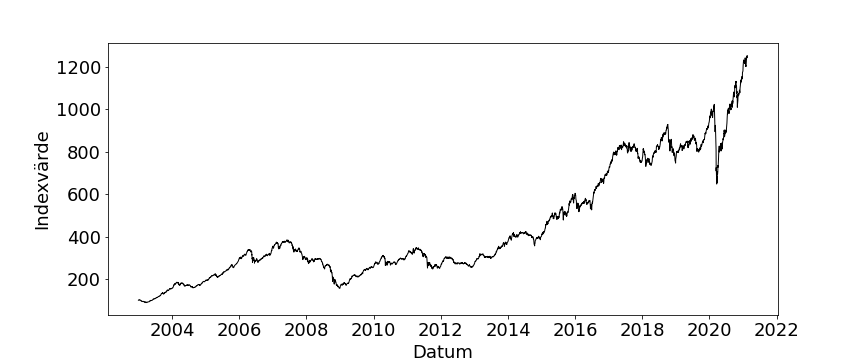
\includegraphics[width=\linewidth]{index.png}
\centering
\end{figure}

\begin{table}[H]
\caption{Deskprivtiv statistik av prisserien}
\begin{adjustbox}{width=1\textwidth}
\begin{tabular}{|c|c|c|c|c|c|c|c|c|c|}
\hline
Index & Start & Slut & N & Min. & Medelvärde & Max. & SD & Skevhet & Kurtosis \\ \hline
OMXSSC   & 2003-01-01 & 2021-02-14 & 4564 & 88.5392  & 436.4533 & 1254.09 & 264.0547 & 0.9545 & -0.2129 \\ \hline
\end{tabular}
\end{adjustbox}
\end{table}

Priserna omvandlades till logaritmerad avkastning enligt ekvation X.Y. I \emph{Figur 4} syns den logaritmerade avkastningsserien där perioder med hög volatilitet kännetecknas av aggressiva prisförändringar. I \emph{Tabell 2} visas sedan deskriptiv statistik. 

\begin{figure}[H]
\caption{Logaritmerad avkastningsserie över perioden}
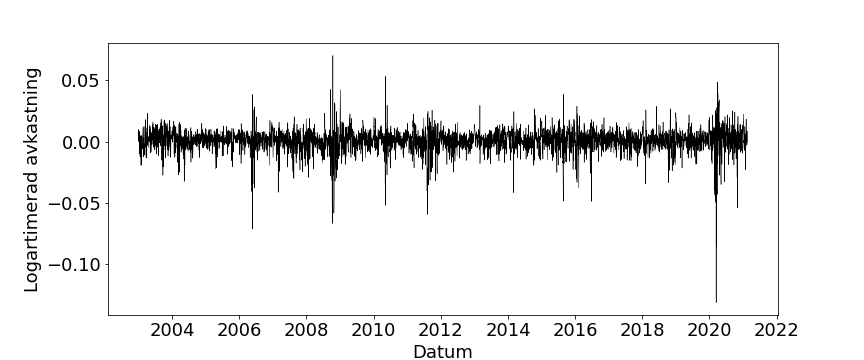
\includegraphics[width=\linewidth]{logreturns.png}
\centering
\end{figure}

\begin{table}[H]
\caption{Deskprivtiv statistik av den logaritmerade avkastningsserien}
\begin{adjustbox}{width=1\textwidth}
\begin{tabular}{|c|c|c|c|c|c|c|c|c|c|}
\hline
Index & Start & Slut & N & Min. & Medelvärde & Max. & SD & Skevhet & Kurtosis \\ \hline
OMXSSC   & 2003-01-01 & 2021-02-14 & 4564 & -0.0875 & 0.0056 & 0.0701 & 0.0006 & -1.4438 & 12.9149 \\ \hline
\end{tabular}
\end{adjustbox}
\end{table}

% Denna känns lite mis placé 
%Skevhetskoefficienten för avkastningsserien är negativ - fördelningen har en lång negativ svans med större frekvens av negativa avkastningar jämfört med positiva avkastningar. Kurtosiskoefficienten är större än tre och kännetecknas av en tjock svans (En: "\emph{fat tail}") där dagar med onormalt hög avkastning förekommer mer frekvent än hos en normalfördelning.

Prediktioner görs $(t=1, 3, 5, 21, 63)$ dagar fram i tiden, där $t=3$ motsvarar en halv börsvecka, $t=5$ en hel börsvecka, $t=21$ en börsmånad och $t=63$ ett börskvartal. Vidare delas 75 procent av datamaterialet in i träningsdata som sträcker sig från 1 januari 2003 till 31 juli 2016. Resterande del av datamaterialet utgörs av testdata som sträcker sig mellan den 3 augusti 2016 till den 14 febuari 2021. 

\subsection{ARMA-GARCH}
En förutsättning för att använda ARMA-GARCH är att tidsserien är stationär. För att testa detta används augmentet Dickey-Fuller test-Fuller-testet genom funktionen som automatiskt väljer optimalt antal laggar baserat på AIC innan testet utförs. För att bekräfta att det specifierade antalet laggar genererar en modell med oberoende residualer görs därefter ett Ljung-Box-test med nollhypotesen att residualerna är oberoende och alternativhypotesen att de inte är oberoende \parencite{box1970distribution}. En annan förutsättning är att feltermerna av en ARIMA är heteroskedastiska, därför görs Lagrange Multiplier-testet på bästa möjliga ARIMA-modell.

Givet att det inte finns belägg för homoskedasticitet väljs sedan bästa möjliga ARMA-GARCH-modell utifrån AIC och BIC. 


\subsection{Long Short-Term Memory (LSTM)}
LSTM har inga formella antaganden och därav finns inga formella test att tillgå, modellen utformas efter ett implicit antagande att det långsiktiga minnet från en period beror på det långsiktigta minnet från perioden innan - att det långsiktiga minnet kan överföras mellan tidsperioderna \parencite{tao2018advanced}.

För att skatta en LSTM behöver modellen så kallade hyperparametrar. Dessa hyperparametrar är olika för olika modeller och alla behöver inte specifieras, i en tidigare studie påpekades det vidare att värdet på hyperparametrarna inte har en väsentlig påverkan på utfallet \parencite{dreyfus2005neural}. Nedan följer de parametrar där det finns andra studier på hur de bör specifieras. Eftersom övriga parametrars specifikation inte ska ha någon väsentlig påverkan har dessa valts utifrån vad som är vanligt förekommande. Antal laggar har valts till lika många som i ARMA-GARCH för jämförbarhetens skull.

Hyperparametrarna med gedigen forskning bakom sig är \emph{loss function, optimizer och epochs}. \par
\emph{Loss function} är ett mått på hur väl modellen presterar på träningsdatan. Förlustfunktionen används som ett mått på modellens fel och detta ska minimeras. MSE (Mean Square Error) rekommenderas för de flesta 'regressionsliknande' modeller, och därför även i detta fall \parencite{purkait2019hands}. \par
\emph{Optimizer} är den typ av algoritm som används för att minimera det ovan beskrivna felet. 'Adam' är en optimeringsalgoritm som visat sig fungera bra för stora dataset och rekommenderas av Purkait \parencite{purkait2019hands}. \par
\emph{Epochs} indikerar antal gånger modellen kommer att itererar genom hela datasetet. Tidigare studier har kommit fram till att valet inte har någon relevant betydelse för hur väl modellen presterar \parencite{siami2018forecasting}. Då Purkait använder fem epoker för LSTM, kommer även denna uppsats använda fem \parencite{purkait2019hands}. \par

\subsection{RMSE och MAPE}
För att mäta hur mycket de skattade stängningspriserna avviker från de verkliga stäningspriserna används RMSE (Root Mean Square Error), som ett mått på medelvärdet av standardfelen. Den bärande egenskapen hos RMSE är att större prediktionsfel får relativt större vikt då måttet baseras på ett viktat medelvärde enligt

\begin{equation}
RMSE = \sqrt{\frac{1}{n}\Sigma_{i=1}^{n}   (\hat{\theta_{t}} - \theta_{t}})^2
\end{equation}

där \emph{n} är det totala antalet observationer, $\theta_{t}$ är den faktiska prisnivån och $\hat{\theta_{t}}$ är den skattade prisnivån under handelsdag \emph{t}. 

Utöver RMSE används även MAPE (Mean Absolute Percentage Error) som har liknande egenskaper som RMSE men mäter de absoluta avvikelserna relativt nivån hos $\theta$, vilket ger de relativa avvikelserna i procent enligt

\begin{equation}
    \textit{MAPE}=\frac{1}{n} 
    \sum_{t=1}^{n} \vert \frac{A_{t}-F_{t}}{A_{t}} \vert \ * 100
\end{equation}

där $A_{t}$ är det aktuella stängningspriset under handelsdag $t$, $F_{t}$ är det predicerade stängningspriset och $n$ är antalet anpassade datapunkter som absolutbeloppet divideras med. Fördelen med MAPE jämfört med RMSE är att den är enklare att begripa tack vare att den är relativ. 




\subsection{Precision, känslighet och F-värde}
För att mäta hur väl modellerna predicerar en stigande respektive fallande prisnivå används en sammanblandningsmatris som registrerar antalet korrekta och inkorrekta klassifikationer \parencite{ModelValidation}. I \emph{Tabell " "} syns en sammanblandningsmatris för den binära klassifikationen.

\begin{table}[H]
\caption{Binär klassifikation}
\scalebox{0.95}{
\begin{tabular}{l|l|c|c|c}
\multicolumn{2}{c}{}&\multicolumn{2}{c}{\textbf{Prediktion}}&\\
\cline{3-4}
\multicolumn{2}{c|}{}&Stigande&Fallande&\multicolumn{1}{c}{}\\
\cline{2-4}
\multirow{2}{*}{\rotatebox{90}{\textbf{Aktuell}}}& Stigande & \emph{Sann stigande (SS)} & \emph{Falskt fallande (FF)} &\\
\cline{2-4}
& Fallande & \emph{Falskt stigande (FS)} & \emph{Sann fallande (SF)} & \\
\cline{2-4}
\end{tabular}}
\end{table}

Tre mått relaterade till sammanblandningsmatrisen är precision, känslighet och F-värde. Måtten ger tillsammans en insikt över hur exakt modellen är. Precision ger svar på frågan 'Hur stor andel av predicerade positiva stiganden är korrekta?' och mäts enligt
\begin{equation}
    \textit{Precision} = \frac{\sum(SS)}{\sum(SS)+\sum(FS)} 
\end{equation}

Känslighet ger svar på frågan 'Hur stor andel av de predicerade uppgångarna var korrekt identifierade?'. Notera att skillnaden mot precision är att precision mäter 'givet att prediktionen var ökat värdet, gick värdet upp?' medan känslighet mäter 'givet att värdet har ökat, var prediktionen korrekt?'. Känslighet mäts genom att dividera antalet korrekt skattade stigande prediktioner med det totala antalet stigande prisnivåer enligt

\begin{equation}
    \textit{Känslighet} = \frac{\sum(SS)}{\sum(SS)+\sum(FF)}
\end{equation}

$F_{\beta}$-värdet är ett mått på exakthet där ett positivt värde ges till faktorn $\beta$ för att värdera antingen precision eller känslighet högst, detta värde defineras som

\begin{equation}
    F_{\beta} = \frac{(\beta^2+1) \textit{Precision} * 
    \textit{Känslighet}}{\beta^2  \textit{Precision} + \textit{Känslighet}}
\end{equation}

För att ge ett balanserat mått viktas precision och känslighet lika med $\beta=1$ \parencite{ModelValidation}. Ett harmoniskt medelvärde mellan de två måttes fås då enligt

\begin{equation}
    \textit{F1} = 2 \Big( \frac{\textit{Precision} * \textit{Känslighet}}{\textit{Precision} + \textit{Känslighet}} \Big)
\end{equation}

Där $F1=1$ är det högsta värdet vilket betyder att modellen inte har några felaktiga predikteringar. $F1=0$ är det lägsta värdet och indikerar att samtliga skattningar om framtida prisnivåer utifrån modellen är felaktiga.


\subsection{Korsvalidering}
Tidsserien korsvalideras med en k-delad korsvalidering som innebär att träning- och testdata flyttas en period framåt från dess ursprungliga startpunkt i $n$ perioder, en procedur som visualiseras nedan i \emph{Figur 5}. Vid nästa period inkluderas alltså det första värdet som predicerades mot i nya träningsdatan \parencite{bergmeir2018note}. I denna studie kommer korsvalideringen utföras över 1000 perioder. 

\begin{figure}[H]
\caption{Illustration av rullande fönster-korsvalidering med fyra perioder.}
\includegraphics[width=0.9\linewidth]{cross_validation.png}
\centering
\end{figure}


Fördelen med denna typ av korsvalidering är att prediktioner görs vid 1000 olika punkter istället för att utgå från en enstaka punkt. Att 1000 perioder görs möjliggör även medelvärdesanalys av valideringsmåtten och på så sätt en statistisk jämförelse mellan dem. För att jämföra måttens medelvärden används z-test då antalet observationer, $n=1000$, ses som tillräckligt.

Låt $a$ motsvara ARMA-GARCH och $b$ LSTM, $i$ vara det valideringsmått som testas och $t$ antal perioder som prediceras framåt i tiden. Då är $\Bar{a}_{i,t}$ ARMA-GARCHs medelvärde för valideringsmått $i$ vid $t$ perioders prediktion, $s_{a,i,t}^2$ variansen och $n_a$ antal observationer. På samma sätt är  $\Bar{b}_{i,t}$ LSTMs medelvärde för valideringsmått $i$ vid $t$ perioders prediktion, $s_{b,i,t}^2$ variansen och $n_b$ antal observationer. Notera dock att $n_a = n_b$. Hypoteserna är som följer. Valet av alternativhypotes beror på om det testas om ARMA-GARCH är högre än LSTM (ekvation 24) eller tvärtom (ekvation 25) för ett givet valideringsmått vid en given prediktionsperiod. 

\begin{equation}
    H_0: \Bar{a}_{i,t} - \Bar{b}_{i,t} = 0 \Leftrightarrow \Bar{a}_{i,t} = \Bar{b}_{i,t}
\end{equation}
\begin{equation}
    H_1: \Bar{a}_{i,t} - \Bar{b}_{i,t} > 0
\end{equation}
\begin{equation}
    H_1: \Bar{a}_{i,t} - \Bar{b}_{i,t} < 0
\end{equation}

med teststatistikan: 

\begin{equation}
    z = \frac{\Bar{a}_{i,t} - \Bar{b}_{i,t} - 0}{\sqrt{\frac{s_{a,i,t}^2}{n_a}+\frac{s_{b,i,t}^2}{n_b}}} \sim N(0,1)
\end{equation}
Som sedan jämförs med det kritiska värdet 1.64 för ett ensidigt test på 5\% signifikansnivå.


\subsection{Handelsstrategi}
För att undersöka hur väl modellerna presterar när de appliceras för att handla med simuleras en handelsstrategi över samma 1000 perioder som i korsvalideringen. I simuleringen är en enhet av index utdistribuerat att handla med utifrån tre kortare tidsperioder ($t=1,3,5$), en medellång ($t=21$) samt en längre tidsperiod på 63 dagar. Handeln utförs och baseras på följande strategier:

\begin{itemize}
    \item Lång strategi: Strategin baseras på att automatiskt öppna en lång position (köpa) när modellen predicerar att prisnivån $t$ dagar fram kommer att stiga.
    \item Kort strategi: Gå kort (sälja) en position när modellen predicerar att prisnivån $t$ dagar fram kommer att falla. 
\end{itemize}

Begränsningen med en enhet medför att två köp- eller säljpositioner i rad inte kan gå igenom, utan den andra  blir då en hållposition. Modellerna jämförs i sin tur med en passiv strategi - att öppna en lång position i index och behålla den utan ytterliggare handlingar. Om modellen lyckas spekulera rätt kring uppgångar och nedgångar om den framtida prisnivån kommer modellen i snitt generera högre avkastning än den passiva strategin. 


%%%%%%%%%%%%%% RESULTAT %%%%%%%%%%%%%%%
\section{Resultat}
\subsection{ARMA-GARCH modellvalidering}
Samtliga resultat i detta avsnitt baseras på den första av de 1000 tidsperioderna som sedan används för korsvalidering. \par

ADF-testet är signifikant med \(p<0.01\). Nollhypotesen att tidsserien inte är stationär förkastas alltså. Optimalt antal laggar (p) var 1 (se bilaga 8.3), vilket även kompletterades med ett insignifikant Ljung-Box-test (se bilaga 8.6). \par

En applikation av ett LM-test på den optimala ARIMA-modellen [ARIMA(1,0,1) = ARMA(1,1)] visar tydliga tecken på heteroskedasticitet, p-värdet är 0.00 (se bilaga 8.4). I tabell 3 följer en sammanställning av ARIMA-modellen. Samtliga parametrar är signifikant skilda från 0 på 5\% nivå. \par

\begin{table}[H]
\centering
\caption{Sammanfattning av ARIMA(1,0,1)}
\begin{tabular}{||llll||}
\hline
              & \textbf{Skattning}  & \textbf{Std. Fel.} & \textbf{p-värde}          \\
              \hline \hline
$\delta$     & 0.0005    & 0.0002    & $0.0087$         \\
$\phi_1$      & 0.6737    & 0.0670    & $<2.2*10^{-16}$  \\
$\theta_1$    & -0.5574   & 0.0754    & $1.42*10^{-13}$  \\ 
\hline \hline
Log likelihood & 11358.46  &           &                  \\
AIC           & -22708.91 &           &                  \\
BIC           & -22683.36 &           &     \\
\hline
\end{tabular}
\end{table}

Eftersom det finns tydliga tecken på heteroskedasticitet applicerades ARMA-GARCH. AIC och BIC visar att ARMA(1,1)-GARCH(1,1) är den bästa möjliga modellen. Nedan följer en sammanställning över denna och i appendix 8.1 finns prediktioner baserat på modellen, inklusive konfidentsintervall, illustrerade. Samtliga parametrar är signifikant skilda från 0 på 5\% signifikansnivå.

\begin{table}[H]
\centering
\caption{Sammanfattning av ARMA(1,1)-GARCH(1,1)}
\begin{tabular}{||llll||}
\hline
              & \textbf{Skattning}  & \textbf{Std. Fel.} & \textbf{p-värde}          \\
              \hline \hline
$\delta$      & 0.0002         & $6.12*10^{-5}$ & 0.0012           \\
$\phi_1$      & 0.7707         & 0.0492         & $<2*10^{-16}$    \\
$\theta_1$    & -0.6484        & 0.0593         & $<2*10^{-16}$    \\
$w$           & $4.16*10^{-6}$ & $5.66*10^{-7}$ & $1.89*10^{-13}$  \\
$\alpha_1$    & 0.1716         & 0.0154         & $<2*10^{-16}$    \\
$\beta_1$     & 0.7721         & 0.0180         & $<2*10^{-16}$    \\ 
\hline \hline
Log likelihood & 11926.87       &                &                  \\
AIC           & -6.9652        &                &                  \\
BIC           & -6.9544        &                &          \\
\hline
\end{tabular}
\end{table}

$\delta, \phi_1$ och $\theta_1$ förekommer även i ARIMA-modellen. Som synes är de annorlunda i ARMA-GARCH. Detta beror på modelleringen av feltermen i GARCH-komponenten ändrar parameterskattningarna.

\subsection{RMSE och MAPE}
I \emph{Tabell 7} sammanfattas resultaten av RMSE och MAPE för de bägge modellerna under den första perioden.

\begin{table}[H]
\caption{RMSE och MAPE vid en period}
\begin{tabular}{||lllllll||}
\hline
                                     &            & \multicolumn{5}{l||}{Tidsperiod}                                  \\
Mått                                 &            & \textbf{1} & \textbf{3} & \textbf{5} & \textbf{21} & \textbf{63} \\ \hline\hline
\multirow{2}{*}{\textbf{RMSE}}  & LSTM       & 1.18          & 4.05         & 4.32          & 20.97           & 150.21        \\
                                & ARMA-GARCH & 0.02          & 7.52         & 9.85          & 2.32            & 43.55           \\ \cline{2-7} 
\multirow{2}{*}{\textbf{MAPE}}  & LSTM       & 0.19\%        & 0.51\%       & 0.39\%        & 0.89\%          & 2.93\%        \\
                                & ARMA-GARCH & 0.004\%        & 0.71\%       & 0.71\%        & 0.54\%          & 1.06\%        \\ \hline
\end{tabular}
\end{table}

Utifrån tabellen syns att LSTM har lägre prediktionsfel än ARMA-GARCH på 3- och 5 dagars sikt medan ARMA-GARCH överträffar LSTM på 1-, 21- och 63 dagars sikt.

Precis som för precision, känslighet och F-värde korsvaliderades RMSE och MAPE över 1000 perioder. Medelvärden av måtten presenteras nedan. 

\begin{table}[H]
\caption{Genomsnittliga RMSE och MAPE över 1000 perioder}
\begin{tabular}{||lllllll||}
\hline
                                     &            & \multicolumn{5}{l||}{Tidsperiod}                                  \\
Mått                                 &            & \textbf{1} & \textbf{3} & \textbf{5} & \textbf{21} & \textbf{63} \\ \hline\hline
\multirow{2}{*}{\textbf{RMSE}}  & LSTM       & 4.97          & 12.16         & 19.82          & 92.26           & 322.02        \\
                                & ARMA-GARCH & 4.91          & 11.90         & 19.18          & 85.88            & 294.07           \\ \cline{2-7} 
\multirow{2}{*}{\textbf{MAPE}}  & LSTM       & 0.61\%        & 0.93\%       & 1.19\%        & 2.75\%          & 5.40\%        \\
                                & ARMA-GARCH & 0.61\%        & 0.91\%       & 1.16\%        & 2.57\%          & 5.02\%        
                                \\ \hline
\multicolumn{5}{l}{\textit{*=P\textless{}0.05}}
\end{tabular}
\end{table}

\subsection{Precision, Känslighet och F-värde}
Nedan ges en sammanfattning över känsligheten, precisionen och F-värdet för de bägge modellerna för varje period.

\begin{table}[H]
\caption{Precision, Känslighet och F-värde}
\begin{tabular}{||lllllll||}
\hline
                                     &            & \multicolumn{5}{l||}{Tidsperiod}                                  \\
Mått                                 &            & \textbf{1} & \textbf{3} & \textbf{5} & \textbf{21} & \textbf{63} \\ \hline\hline
\multirow{2}{*}{\textbf{Precision}} & LSTM       & 1          & 0.33       & 0.60       & 0.60        & 0.53        \\
                                     & ARMA-GARCH & 1          & 0.33       & 0.60       & 0.62        & 0.59        \\ \cline{2-7} 
\multirow{2}{*}{\textbf{Känslighet}}  & LSTM       & 1          & 1          & 1          & 0.92           & 0.73       \\
                                     & ARMA-GARCH & 1          & 1          & 1          & 1           & 1           \\ \cline{2-7} 
\multirow{2}{*}{\textbf{F-värde}}    & LSTM       & 1          & 0.5        & 0.75       & 0.73       & 0.61       \\
                                     & ARMA-GARCH & 1          & 0.5        & 0.75       & 0.77       & 0.74        \\ \hline
\end{tabular}
\end{table}

Modellerna ger snarlika resultat upp till 21 perioder. Det beror på att båda uppfattar en positiv trend i prisutvecklingen under det spannet. Vid 63 perioder signalerar LSTM dock en fallande prisnivå under delar av intervallet (se bilaga 8.1), vilket medför att dess värden blir något lägre än ARMA-GARCH. Värt att notera är att känsligheten är 1 för samtliga tidsperioder hos ARMA-GARCH, vilket beror på att modellen predicerar stigande i alla tidsperioder (t=1, ..., t=63).

För att säkerställa att resultaten ovan inte enbart är en effekt av den valda tidpunkten gjordes korsvalidering över 1000 perioder. I \emph{Tabell 6} sammanfattas resultaten.

\begin{table}[H]
\caption{Precision, Känslighet och F-värde över 1000 perioder}
\begin{tabular}{||lllllll||}
\hline
                                     &            & \multicolumn{5}{l||}{Tidsperiod}                                  \\
Mått                                 &            & \textbf{1} & \textbf{3} & \textbf{5} & \textbf{21} & \textbf{63} \\ \hline\hline
\multirow{2}{*}{\textbf{Precision}} & LSTM       & 0.22*          & 0.50       & 0.52       & 0.53        & 0.57        \\
                                     & ARMA-GARCH & 0.001          & 0.52       & 0.55       & 0.57*        & 0.57        \\ \cline{2-7} 
\multirow{2}{*}{\textbf{Känslighet}}  & LSTM       & 0.22*          & 0.59          & 0.63          & 0.36           & 0.38      \\
                                     & ARMA-GARCH & 0.001          & 0.59          & 0.76*          & 0.94*           & 0.98*           \\ \cline{2-7} 
\multirow{2}{*}{\textbf{F-värde}}    & LSTM       & 0.22*          & 0.51        & 0.53       & 0.37       & 0.43        \\
                                     & ARMA-GARCH & 0.001          & 0.53        & 0.61*       & 0.71*       & 0.72*        \\ \hline
\multicolumn{5}{l}{\textit{*=P\textless{}0.05}}
\end{tabular}
\end{table}

LSTM är statistiskt signifikant bättre avseende samtliga tre mått vid en periods prediktion, medan ARMA-GARCH är överträffar LSTM avseende känslighet och F-värde på 5, 21 och 63 perioders prediktion, samt har högre precision på 21 perioders sikt.


\subsection{Utvärdering av handelsstrategi}
För utvärdering av handelsstrategin jämförs hur stor procentuell avkastning modellerna genererat under varje givet tidsintervall. I \emph{Tabell 9} presenteras den procentuella avkastningen av att handla med respektive strategi samt hur många positioner algoritmen öppnat under de 1000 perioderna. För att kunna utvärdera strategierna används den passiva investeringsstrategin som riktmärke - en strategi som genererat 61.9\% avkastning över perioden.

\begin{table}[H]
\centering
\caption{Avkastning över 1000 perioder}
\begin{adjustbox}{width=1\textwidth}
\begin{tabular}{||llcccccc||}
\hline
                                     &            & \multicolumn{6}{l||}{Tidsperiod}                                  \\
Modell                                 &            & \textbf{1} & \textbf{3} & \textbf{5} & \textbf{21} & \textbf{63} & \textbf{1000}\\ \hline\hline
\multirow{2}{*}{\textbf{LSTM}}  & Avkastning       & 12.53\%          & -0.42\%         & 7.69\%          & 24.18\%           & 8.26\%  & -     \\
                                & Antal positioner & 51          & 87         & 121          & 137            & 188 &  -        \\ \cline{2-8} 
\multirow{2}{*}{\textbf{ARMA-GARCH}}  & Avkastning       & 117.9\%        & 117.05\%       & 112.64\%        & 92.27\%          & 59.3\%       & - \\
                                & Antal positioner & 78        & 62       & 54        & 5          & 2     &   -
                                \\ \cline{2-8}
{\textbf{Passiv strategi}} & Avkastning &- &- &- &- &- & 61.90\% \\ \hline
\end{tabular}
\end{adjustbox}
\end{table}

Ur tabellen går det att utröna att LSTM presterar sämre än den passiva strategin oavsett vilken tidsperiod prediktionerna baseras på. ARMA-GARCH presterar bättre än den passiva strategin på en till 21 perioders sikt och sämre därefter. Utifrån dessa resultat tyder det på att ARMA-GARCH överträffar LSTM vid implementation av ovan nämnda handelsstrategier. 


\section{Diskussion}
Denna studie ämnade att undersöka om djupinlärningsmodeller med fördel kan användas istället för traditionella ekonometriska modeller på svenskt börsindex. Därutöver undersöks om en handelsstrategi som är bättre än indexet kan byggas baserat på någon av modellerna. För att besvara dessa användes de tre olika validergstyperna

\begin{itemize}
    
\item Prediktionsfel (MAPE och RMSE)

\item Binär klassificering (F-värde, precision och känslighet)

\item Simulerad handel 
\end{itemize}

De två förstnämnda undersöktes först vid en enskild period för att sedan korsvalideras över 1000 perioder. Simuleringen av handel gjordes enbart över 1000 perioder. Baserat på resultatet i avsnittet ovan, vilken modell är bäst lämpad och går det att bygga en lönsam handelsstrategi på någon av dem?

Rörande prediktionsfel, mätt med RMSE och MAPE, indikerade resultatet vid en enskild period att LSTM skulle vara bättre vid tre och fem perioder och ARMA-GARCH vid en, 21 och 63 perioder. Då det enbart är vid en enskild tidpunkt är det svårt att avgöra om skillnaderna är permanenta eller enbart en konsekvens av den punkt på tidsserien där prediktionerna gjordes, vilket var varför korsvalidering över 1000 perioder gjordes. Den analysen visar att ingen av modellerna är signifikant bättre än den andra oavsett tidsperiod. Slutsatsen blir således att ingen av modellerna är att föredra över den andra om validering görs utifrån prediktionsfel. 

Den binära klassificeringen av prisupp - och nedgångar utgörs av känslighet, precision och F-värde. \textit{Känslighet} ger svar på frågan "Hur stor andel av faktiska uppgångar var korrekt identifierade?". Vid en enskild tidpunkt är måtten identiska upp till 5 perioder. Vid 21 och 63 perioder är ARMA-GARCH bättre. Det mer intressanta är såklart prestationen över 1000 perioder. Även om resultatet inte är tillfredsträllade visar LSTM mer exakta prediktioner en tidsperiod fram, då enbart i snitt 22 procent av faktiska uppgångar identifieras korrekt. Detta är visserligen avsevärt bättre än en ARMA-GARCH med 0.1 procent korrekt skattade. Modellerna är oskiljbara på 3 perioder sikt, då båda identifierar uppgångar i snitt 59 procent av fallen. ARMA-GARCH är signifikant bättre på 5, 21 och 63 perioders sikt. Båda modellerna är bättre än slumpen på 5 perioders sikt men på 21 och 63 dagars sikt faller LSTM till att enbart identifiera i snitt 36 procent respektive 38 procent av uppgångarna. I stark kontrast till det identifierar ARMA-GARCH i snitt 94 procent respektive 98 procent av uppgångarna. Sammantaget är alltså LSTM att föredra på kort sikt och ARMA-GARCH på medel- till lång sikt.

\textit{Precision} ger svaret på frågan 'Vilken andel av predicerade positiva stiganden var korrekta?'. Vid en enskild period presterar överlag modellerna jämförbart, det finns en liten fördel till ARMA-GARCH över 21 och 63 perioder. Över 1000 perioder går det precis som med känslighet att utröna att LSTM är bättre på en dags sikt. Att värdena är identiska med känslighet beror på att testen testar samma sak vid en period. Antingen är det en sann stigande och då ger bägge måtten 1 eller så är det inte sant stigande och då returnerar båda måtten 0 (se ekvation 13 och 14). På 21 perioders sikt är ARMA-GARCH bättre, i övrigt är modellerna inte åtskiljbara. Det intressanta är att här, såväl som med känslighet, är LSTM bättre på en periods sikt. LSTM är alltså bättre på att identifiera uppgångar såväl som att andelen korrekta stigande prediktioner är högre på en periods sikt. Återigen är medelvärdet inte särskilt imponerande, enbart 22\% av predicerade stiganden är i snitt korrekta, vilket är avsevärt sämre än att slumpmässigt gissa. På längre sikt är i snitt drygt 50\% av förutspådda uppgångar korrekta, oavsett modell. Alltså knappt bättre än att slumpmässigt gissa. 

\textit{F-värdet} mäter testets exakthet och är en sammanvägning av precision och känslighet. Vid en enskild period är modellerna jämförbara upp till 5 perioder, sedan är ARMA-GARCH bättre. Över 1000 perioder framgår återigen att LSTM är bättre på en periods sikt, medan ARMA-GARCH är på 5, 21 och 63 dagars sikt. Slutsatsen är att LSTM är mer noggrann på en dags sikt, ARMA-GARCH är noggrannare på 5, 21 och 63 dagars sikt. 

Resultaten från den sista valideringstypen, simulerad handling över 1000 perioder, visade entydigt i att ARMA-GARCH är att föredra oavsett hur långt in i framtiden man vill förutspå. Det är även tydligt, och föga förvånande, att kortsiktiga prediktioner är mer lönsamma än långsiktiga. ARMA-GARCH är även bättre än den passiva strategin upp till 21 perioders prediktion medan LSTM är sämre oavsett prediktionsperiod. Som tidigare diskuterades kan den passiva strategin liknas vid en slumpvandring, och givet att EMH råder ska det därför inte gå att finna en modell som är bättre än den denna. Men eftersom ARMA-GARCH visar sig generera högre avkastning än den passiva strategin kan EMH alltså förkastas under den studerade perioden. En ARMA-GARCH kan alltså användas för att applicera en algoritmisk handelsstrategi som överpresterar index. 

Intressant är också att modellerna var oskiljbara rörande prediktionsfel men skillnaden i avkastning är stor. Ur ett bredare perspektiv kan dessa resultat tänkas påvisa att en modell som presterar väl på modellvalideringen inte nödvändigtvis är samma modell som genererar högst avkastning. Det belyser vikten av att inte enbart basera modellval på lägsta möjliga prediktionsfel. 

När resultatet av diskussionen ovan sammanfattas går det att dra slutsatsen att modellerna är oskiljbara om målet är att minimera prediktionsfel oavsett tidsperiod. För den som är intresserad av att ta köp eller säljbeslut är LSTM att föredra på kort sikt (en period) och ARMA-GARCH på medel till lång sikt (5, 21 och 63 dagar). Om målet snarare är att maximera avkastning är ARMA-GARCH att föredra. \emph{Tabell 7} illustrerar dessa slutsatser.

\begin{table}[H]
\caption{Sammanfattning av modellernas användbarhet}
\begin{adjustbox}{width=1\textwidth}
\begin{tabular}{||llll||}
\hline
& \multicolumn{3}{l||}{Mål} \\
Tidsperioder framåt & \textbf{Prediktionsfel} & \textbf{Exakthet} & \textbf{Avkastning}\\ \hline\hline
{\textbf{Kort (1)}} & Oskiljbara          & LSTM & ARMA-GARCH\\ \cline{2-4} 
{\textbf{Medelkort (3)}} & Oskiljbara          & Oskiljbara & ARMA-GARCH\\ \cline{2-4} 
{\textbf{Medel (5)}}       & Oskiljbara        & ARMA-GARCH & ARMA-GARCH\\ \cline{2-4}
{\textbf{Medellång (21)}}       & Oskiljbara        & ARMA-GARCH & ARMA-GARCH\\ \cline{2-4}
{\textbf{Lång (63)}}       & Oskiljbara        & ARMA-GARCH & ARMA-GARCH \\
\hline
\end{tabular}
\end{adjustbox}
\end{table}

Flera tidigare studier nådde samstämmigt slutsatsen att LSTM är åtminstone lika bra och ofta bättre än ARIMA. Att denna studie visat andra resultat kan tänkas bero på tre olika faktorer. För det första har ett flertal tidigare studier applicerat ARIMA utan GARCH-komponent för att jämföra LSTM med. Men som diskuterades tidigare och som påvisades i denna studie, är antagandet om homoskedasticitet sällan uppfyllt inom finansiell analys. Att använda en ARIMA-modell utan GARCH-komponent är således suboptimalt. En andra faktor som kan ha påverkat är specifikationen av LSTM-modellen. Denna studie valde att låta modellen använda en lagg, eftersom det är jämförbart med vad som var bästa möjliga ARMA-GARCH. Väljer man däremot att använda fler laggar kan man i teorin få ett bättre resultat. Dock ökar risken för en överanpassning av data markant -  modellen anpassas för nära till den befintliga datan vilket i sin tur hämmar dess möjlighet att förutspå utanför det befintliga urvalet. I denna uppsats valdes en specifikation baserat på teori snarare än empiri, vilket med fördel kan minska risken för överanpassning men kan å andra sidan ha gjort resultaten mindre fördelaktiga för LSTM-modellen. Den tredje faktorn är att det i denna studie har säkerställts att samtliga ARMA-GARCHs antaganden är uppfyllda. Detta har visat sig inte alltid vara fallet i andra studier \parencite{paliwal2009neural}. 

Ses modellerna ur ett användarvänlighetsperspektiv är ARMA-GARCH att föredra då LSTM är svårtolkad och som påpekades i metoden finns det inte särskilt gedigen forskning bakom hur modellerna ska specifieras. Modellen är icke-parametrisk och det går således inte heller att dra slutsatser kring specifika variablers signifikans. En fördel med LSTM är dock att den bara har ett antagande att uppfylla, vilket gör den enkel att applicera. 

\subsection{Felkällor}
Det finns det flera potentiella felkällor till alla tidsseriemodeller \parencite{hyndman2018forecasting}. Den slumpmässiga feltermen, benämnd \(e_t\), är såklart en av dem. Denna uppsats, och de flesta andra på området, försöker aktivt motverka denna. Det finns dock åtminstone tre ytterligare felkällor som är svårare att aktivt motverka. 

Den första är estimaten av parametrar i modellerna i såväl ARMA-GARCH som LSTM. Exempelvis har denna uppsats valt att välja ARMA-GARCH-modell baserat på AIC och BIC, men andra liknande mått för utvärdering finns som hade kunnat ge annorlunda resultat. Hannan-Quinn Information Criterion (HQC) är ett sådant \parencite{hannan1979determination}. På samma vis hade LSTM-modellen kunnat specifieras annorlunda, med viss försiktighet rörande överanpassning hade denna studie kunnat optimera de använda parametrarna till detta dataset och på så vis fått andra estimat. 

Den andra är valet av modell. Det finns andra typer av GARCH-modeller att tillgå, däribland exponentiell GARCH (EGARCH) som används inom finansiell analys \parencite{nelson1991conditional}. ARMA-komponenten hade exempelvis kunnat bytas ut mot ARFIMA (Autoregressive Fractionally Integrated Moving Average), som visat sig effektiva när tidsserier behöver ha ett långt minne, precis som LSTM \parencite{taqqu1995estimators}. Angående LSTM hade det varit möjligt att använda en mer simpel modell. Neurala nätverk, som LSTM är en underkategori till, används frekvent inom området \parencite[se t.ex.][]{rather2015recurrent, li2010applications}. Det finns även andra typer av LSTM, såsom 'Deep LSTM' med flera lager av neuroner \parencite[se applikation i][]{hansson2017stock}. Vidare baserades valet av modell i samtliga perioder av korsvalideringen på vilken modell som var bäst vid sista träningsperioden. Andra resultat hade möjligen kunnat nås om modellen vid varje enskild tidpunkt modellerades om och parametrarna optimerades utifrån den nya datapunkten som tillförts. Det är inte heller säkert, även om det är troligt, att alla modellantaganden uppfylls i alla av de 1000 perioderna vilket kan påverkat hur väl ARMA-GARCH presterat.  

Slutligen gäller inte nödvändigtvis förutsättningarna som var när datan samlades in, in i framtiden. Ett extremt exempel på denna felkälla är Bitcoin. I maj 2016 var en Bitcoin värd ungefär 450 USD, fem år senare, när denna uppsats skriv i maj 2021, är en Bitcoin värd ungefär 64000 USD. En ökning med över 14000\% \parencite{yahoo_bitcoin}. Det förefaller osannolikt att en modell som var bra då fortfarande håller måttet. Poängen är alltså att framtida applikationer av de modeller som använts i denna studie inte nödvändigtvis genererar samma resultat.


%%%%%%%%%%%%%%%%%%% SLUTSATS %%%%%%%%%%%%%%%%%%%
\section{Slutsats}
Denna studie ämnade att besvara frågorna 'Kan en djupinlärningsmodell med fördel användas som substitut för tradtionella ekonometriska metoder på svenskt börsindex?' samt 'Kan en algoritmisk handelsstrategi som är bättre än indexets utveckling byggas?'. Resultatet har visat att om minimering av prediktionsfel är målet är modellerna lika kapabla. Om målet snarare är exakthet (noggrannhet) är LSTM att föredra på en periods sikt och ARMA-GARCH vid fem eller fler perioders sikt. Oavsett tidsperiod är ARMA-GARCH att föredra för den som vill använda modellerna för att generera högsta möjliga avkastning. ARMA-GARCH kan även användas för att bygga en handelsstrategi som är bättre än indexets utveckling.

Vidare studier kan med fördel undersöka om resultaten håller för andra index än OMXSSC. Detta vore intressant eftersom slutsatserna av denna uppsats delvis går emot tidigare forskning. Som diskuterades i felkällor kan framtida studier även djupdyka i olika varianter av ARMA-GARCH (såsom ARFIMA-EGARCH) respektive LSTM-modell (såsom Deep LSTM) och jämföra dessa.



%%%%%%%%%%%%%%%%%%% BILAGOR %%%%%%%%%%%%%%%%%%%
\newpage
\section{Bilagor}

\subsection{Bilaga 1 - Prediktioner vid t=1}
\begin{figure}[H]
\caption{LSTM-prediktioner vid enskild tidpunkt}
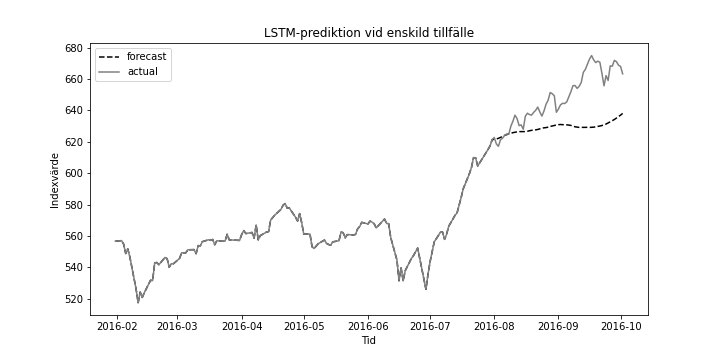
\includegraphics[width=\linewidth]{lstm_pred.png}
\centering
\end{figure}
Notera att LSTM inte har konfidensintervall.

\begin{figure}[H]
\caption{ARMA-GARCH-prediktioner vid enskild tidpunkt}
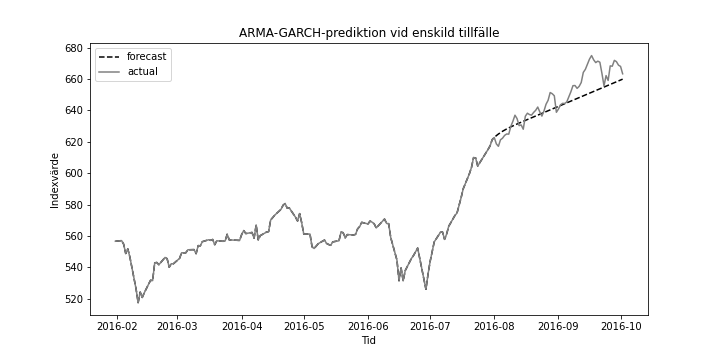
\includegraphics[width=\linewidth]{arma_garch_pred.png}
\centering
\end{figure}

\begin{figure}[H]
\caption{ARMA-GARCH-prediktioner vid enskild tidpunkt med prediktionsintervall}
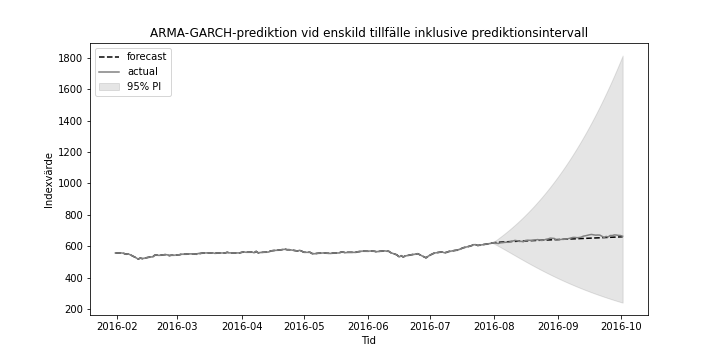
\includegraphics[width=\linewidth]{arma_garch_pred_interval.png}
\centering
\end{figure}



\subsection{Bilaga 2 - Histogram över logaritmerad avkstning}
\begin{figure}[H]
\caption{Histogram logaritmerad avkastning}
\includegraphics[width=\linewidth]{histogram.png}
\centering
\end{figure}


\subsection{Bilaga 3 - ADF-test}
\begin{figure}[H]
\caption{ADF-test med optimalt antal laggar}
\includegraphics[width=0.8\linewidth]{adf.png}
\centering
\end{figure}


\subsection{Bilaga 4 - LM-test}
\begin{figure}[H]
\caption{LM-test för heteroskedasticitet}
\includegraphics[width=0.8\linewidth]{lm_test.png}
\centering
\end{figure}


\subsection{Bilaga 5 - AIC och BIC för ett urval av modeller}
Ju lägre värde, desto bättre. ARMA(1,1)-GARCH(1,1) ger lägst resultat.
\begin{table}[H]
\caption{AIC och BIC för olika parametervärden på ARMA-GARCH}
\begin{tabular}{||lll||}
\hline
& \multicolumn{2}{l||}{Kriteria} \\
ARMA(p,q)-GARCH(p,q) & \textbf{AIC} & \textbf{BIC}\\ \hline\hline
{\textbf{(0,0)-(1,0)}} & -6.782  & -6.777 \\ \cline{2-3} 
{\textbf{(0,0)-(1,1)}} & -6.938  & -6.931 \\ \cline{2-3}
{\textbf{(0,1)-(1,1)}} & -6.951  & -6.942 \\ \cline{2-3} 
{\textbf{(1,0)-(1,1)}} & -6.954  & -6.944 \\ \cline{2-3} 
{\textbf{(1,1)-(1,1)}} & \textbf{-6.965}  & \textbf{-6.954} \\ \cline{2-3} 
{\textbf{(1,1)-(2,1)}} & -6.965  & -6.952 \\ \cline{2-3} 
{\textbf{(1,1)-(2,2)}} & -6.964  & -6.950 \\ \cline{2-3}
{\textbf{(2,1)-(2,2)}} & -6.964  & -6.948 \\ \cline{2-3} 
{\textbf{(2,2)-(2,2)}} & -6.963  & -6.946 \\ \hline
\end{tabular}
\end{table}


\subsection{Bilaga 6 - Ljung-Box Test för ARIMA(1,0,1)}
\begin{figure}[H]
\caption{Ljung-Box-test med 1 lag}
\includegraphics[width=0.8\linewidth]{ljung-box.png}
\centering
\end{figure}


\subsection{Bilaga 7 - Python- och R-paket}
Följande paket användes i Python version 3.8 respektive R version 4.0 för att skapa modellerna. 

\textbf{R} \par
\textit{forecast} användes för att skapa ARIMA-modellen. \par
\textit{aTSA} användes för att testa för heteroskedasticitet. \par
\textit{fGarch} användes för att skapa ARMA-GARCH-modellen. \par
\textit{urca} användes för ADF-Fuller-testet. \par
\textit{stats} användes bl.a. för Ljung-Box-test. \par

\textbf{Python} \par
\textit{Scikit-learn} och \textit{Keras} användes för att skapa LSTM-modellen.


\subsection{Bilaga 8 - Indexbeståndsdelar 12 februari 2021}

\begin{table}[H]
\scalebox{0.62}{
\begin{tabular}{|l|l|l|l|}
\hline
Namn & Kortnamn & Namn & Kortnman \\ \hline
\rowcolor[HTML]{EFEFEF} 
Abliva AB & ABLI & Magnolia Bostad AB & MAGNO \\ \hline
Actic Group AB & ATIC & Maha Energy AB & MAHAa \\ \hline
\rowcolor[HTML]{EFEFEF} 
Active Biotech AB (publ) & ACTI & Malmbergs Elektriska AB (publ) & MEABb \\ \hline
Alligator Bioscience AB & ATORX & Medivir AB & MVIRb \\ \hline
\rowcolor[HTML]{EFEFEF} 
Anoto Group AB & ANOT & Micro Systemation AB (publ) & MSABb \\ \hline
Arctic Paper SA & ARP & Midway Holding AB & MIDWb \\ \hline
\rowcolor[HTML]{EFEFEF} 
Arise AB & ARISE & Midway Holding AB & MIDWa \\ \hline
Ascelia Pharma AB & ACELP & Moberg Pharma AB (publ) & MBPH \\ \hline
\rowcolor[HTML]{EFEFEF} 
Atvexa AB & ATVEXAb & Moment Group AB & MOMENT \\ \hline
B3 Consulting Group AB (publ) & B3 & MultiQ International AB & MULQ \\ \hline
\rowcolor[HTML]{EFEFEF} 
BE Group AB (publ) & BEGR & Nelly Group AB (publ) & NELLY \\ \hline
Beijer Electronics Group AB & BELE & Net Insight AB & NETIb \\ \hline
\rowcolor[HTML]{EFEFEF} 
Bergs Timber AB (publ) & BRGb & NGS Group AB & NGSG \\ \hline
BioInvent International AB & BINV & Nilorngruppen AB & NILb \\ \hline
\rowcolor[HTML]{EFEFEF} 
Bjorn Borg AB & BORG & Note AB (publ) & NOTE \\ \hline
Bong AB & BOLJ & Novotek AB & NTEKb \\ \hline
\rowcolor[HTML]{EFEFEF} 
Boule Diagnostics AB & BOUL & Odd Molly International AB & ODD \\ \hline
C Rad AB & CRADb & Ortivus AB & ORTIb \\ \hline
\rowcolor[HTML]{EFEFEF} 
Christian Berner Tech Trade AB & CBTTb & Ortivus AB & ORTIa \\ \hline
Concejo AB (publ) & CNCJOb & Oscar Properties Holding AB & OP \\ \hline
\rowcolor[HTML]{EFEFEF} 
Concordia Maritime AB & CCORb & Poolia AB & POOLb \\ \hline
Dedicare AB (publ) & DEDIC & Precise Biometrics AB & PREC \\ \hline
\rowcolor[HTML]{EFEFEF} 
Doro AB & DORO & Prevas AB & PREVb \\ \hline
Duroc AB & DURCb & Profilgruppen AB & PROFb \\ \hline
\rowcolor[HTML]{EFEFEF} 
Egetis Therapeutics AB (publ) & EGTX & Projektengagemang Sweden AB & PENGb \\ \hline
Electra Gruppen AB (publ) & ELEC & Qliro AB & QLIRO \\ \hline
\rowcolor[HTML]{EFEFEF} 
Elos Medtech AB & ELOSSb & Railcare Group AB & RAILG \\ \hline
Empir Group AB & EMPIRb & Rnb Retail and Brands AB (publ) & RNBS \\ \hline
\rowcolor[HTML]{EFEFEF} 
Endomines AB (publ) & ENDO & Saniona AB & SANION \\ \hline
Eniro AB & ENRO & Semcon AB & SEMC \\ \hline
\rowcolor[HTML]{EFEFEF} 
Episurf Medical AB & EPISb & Sensys Gatso Group AB & SENS \\ \hline
Etrion Corp & ETRN & SERNEKE Group AB (publ) & SRNKEb \\ \hline
\rowcolor[HTML]{EFEFEF} 
Ework Group AB & EWRK & SinterCast AB & SINT \\ \hline
Feelgood Svenska AB (publ) & FEEL & Softronic AB & SOFb \\ \hline
\rowcolor[HTML]{EFEFEF} 
FM Mattsson Mora Group AB & FMMb & Starbreeze AB & STZEb \\ \hline
FormPipe Software AB & FPIP & Starbreeze AB & STZEa \\ \hline
\rowcolor[HTML]{EFEFEF} 
Gaming Innovation Group Inc & GIGSEK & Stockwik Forvaltning AB & STWK \\ \hline
GHP Specialty Care AB & GHP & Strax AB & STRAX \\ \hline
\rowcolor[HTML]{EFEFEF} 
Green Landscaping Group AB & GREENL & Studsvik AB & SVIK \\ \hline
Hanza Holding AB & HANZA & Svedbergs i Dalstorp AB & SVEDb \\ \hline
\rowcolor[HTML]{EFEFEF} 
Image Systems AB & ISY & TradeDoubler AB & TRAD \\ \hline
Immunicum AB & IMMUN & Vicore Pharma Holding AB & VICOR \\ \hline
\rowcolor[HTML]{EFEFEF} 
Irras AB & IRRAS & Viking Supply Ships AB & VSSABb \\ \hline
Josemaria Resources Inc & JOSE & Wise Group AB & WISE \\ \hline
\rowcolor[HTML]{EFEFEF} 
KABE Group AB & KABEb & Xbrane Biopharma AB & XBRANE \\ \hline
Karolinska Development AB & KDEV & ZetaDisplay AB & ZETA \\ \hline
\rowcolor[HTML]{EFEFEF} 
Lammhults Design Group AB & LAMMb & \multicolumn{2}{l|}{\cellcolor[HTML]{EFEFEF}} \\ \hline
\end{tabular}}
\end{table}





\newpage
\printbibliography
\end{document}